\section{Theorie}
\subsection{Vakuum}
Hingegen der allgemeinen Auffassung, dass Vakuum ein Volumen gänzlich ohne Materie beschreibt, wird in der Physik und Technik
der Vakuumbegriff in Bereiche eingeteilt.
Abhängig vom Druck, der mittleren freien Weglänge und des Strömungsverhaltens lassen sich, wie Tabelle $\ref{tab:bereiche}$ zeigt, vier Bereiche unterscheiden.

\begin{table}[!hht]
\begin{tabular}{c c c c}
 Bereich & Druck $\:/\: mbar$ & freie Weglänge $\:/\: m$ & Strömungsmechanismus \\
 \midrule
 Grobvakuum & 1000 - 1 & $10^{-7}$ - $10^{-4}$ & viskos \\
 Feinvakuum & 1 - $10^{-5}$ & $10^{-4}$ - $10^{-1}$ & Knudsen \\
 Hochvakuum & $10^{-3}$ - $10^{-7}$ & $10^{-1}$ - $10^3$ & molekular \\
 Ultrahochvakuum & $< 10^{-7}$ & $> 10^3$ & molekular \\
\end{tabular}
\caption{Bereichseinteilung des Vakuums}
\label{tab:bereiche}
\end{table}

Die mittlere freie Weglänge beschreibt die durchschnittliche Wegstrecke, die ein Teilchen zurücklegt, ohne mit anderen Teilchen in Wechselwirkung zu treten.
Eben für Gase und der Annahme, dass eine Maxwellsche Geschwindigkeitsverteilung vorliegt, gilt die Gasgleichung
\begin{equation}
  \lambda = \frac{k_B T}{\sqrt{2}\pi d^2p}.
\end{equation}
Hierbei ist $k_B$ die Boltzmann-Konstante, $T$ die Temperatur, $d$ der Durchmesser des Moleküls und $p$ der Druck.
\subsection{Strömungsarten}
Für die Charakterisierung einer vorliegenden Strömung und für die Wahl der richtigen Pumpe wird die Knudsen-Zahl $K_n$ als einheitenlose Größe verstanden.
Sie ist definiert durch den Quotienten der mittleren freien Weglänge $\lambda$ und der charakteristischen Länge der Strömung $l_c$
\begin{equation}
  K_n=\frac{\lambda}{l_c}.
\end{equation}
Bei einer Knudsen-Zahl $K_N < 0,01$ wird von einer Kontinuumsströmung und Grobvakuum gesprochen. Hierbei kommt es vermehrt zum Zusammenstoßen der Teilchen im Gas
untereinander. Die mittlere freie Weglänge ist kleiner als die Abmessung des Strömungskanals.
Es wird außerdem in laminarer und turbolenter Strömung unterschieden.
Die laminare Strömung beschreibt Strömungen in Schichten. Die Gasteilchen bleiben immer parallel zueinander.
Nimmt die Strömungsgeschwindigkeit aber zu, so lösen sich die Schichten auf und die Strömung wird turbolent.
Beschrieben wird der Grenzübergang durch die Reynoldszahl
\begin{equation}
  R=\frac{\rho v l_c}{\eta}.
\end{equation}
$\rho$ ist die Dichte, $v$ ist die Strömungsgeschwindigkeit und $\eta$ die dynamische Viskosität.
Turbolente Strömungen kommen zum Beispiel beim Abpumpen von Atmosphärendruck auf.
In der Pumptechnik wird versucht, diese Strömungsart zu verhindern, da durch auftretende Strömungswiderstände, Pumpen mit erhöhter Saugkraft benötigt werden.\newline
Für $ 0,01 \leq K_n \leq 0,5$ wird der Begriff der Knudsen-Strömung gebraucht.
Charakteristisch ist diese für den Feinvakuumbereich, der in technischen Anwendungen häufig eine Rolle spielt.\newline
Liegt die Knudsen-Zahl oberhalb von 0,5 so lassen sich kaum noch Wechselwirkungen der Gasteilchen untereinander feststellen.
Es kommt zur molekularen Strömung, bei der die mittlere freie Weglänge sehr viel größer als die Abmessung des Strömungskanals ist.
\subsection{Ideales Gas}
In der Thermodynamik wird das Modell des idealen Gases als idealisierte Vereinfachung für die Beschreibung von Gasprozessen verwendet.
Wechselwirkungen treten ausschließlich durch elastische Stöße der Teilchen untereinander und durch Stöße mit der Wand auf.
Das ideale Gas ist vom Druck $p$, dem Volumen $V$, der Teilchenzahl $N$ und der Temperatur $T$ abhängig und die Zustandsgleichung
folgt zu
\begin{equation}
pV=N k_B T.
\label{eq:idealesgas}
\end{equation}
Nach dem Gesetz von Boyle-Mariotte ist der Druck unter $T=const$ antiproportional zum Volumen.
Diese Aussage der Zustandsgleichung des idealen Gases ist von Bedeutung für den später beschriebenen Versuch.
\subsection{Saugvermögen}
Das Saugvermögen $S$ einer Pumpe gibt den geförderten Volumenstrom an.
Ausdrückbar ist dieser über den gemessenen Druck über die Zeit $p(t)$.\\
Getroffen werden müssen folgende Annahmen:
\begin{itemize}
  \item Bei der Messung gilt $V=const$.
  \item Das beförderte Gas kann als ideales Gas angesehen werden.
  \item Bei der Messung gilt außerdem $T_\text{Gas}=const$.
  \item Das Gas befindet sich zu jedem Zeitpunkt im thermodynamischen Gleichgewicht.
  \item Es tritt keine Desorption auf.
  \item Das Saugvermögen ist konstant und unabhängig vom Druck.
\end{itemize}
Um einen Zusammenhang zwischen dem Druck $p$ und dem Saugvermögen $S$ zu erhalten, wird die Kolbenpumpe als einfachste Pumpenart verwendet,
um durch konstante Kolbengeschwindigkeit auf $\dot{V}=S$ zu kommen.
Durch Ableiten der Zustandsgleichung des idealen Gases $\ref{eq:idealesgas}$ erhält man die Differentialgleichung
\begin{equation}
  \dot{p}V=-pS,
\end{equation}
wodurch man nach Lösen
\begin{equation}
  p(t)=p_0 e^{\frac{-tS}{V}}
\end{equation}
erhält.\\
Berücksichtigt werden muss ebenso, dass es einen endlichen Enddruck gibt.
Er muss aufgrund von allseits auftretenden Leckagen und des Ausgasens durch die Innenwände , den sogenannten virtuellen Lecks, existieren.
\subsection{Leckrate}
Für die spätere Auswertung ist ebenso die Definition der Leckrate $Q$ wichtig. Es gilt
\begin{equation}
  S=\frac{Q}{p_\text{G}},
  \label{eq:leckrate1}
\end{equation}
wodurch
\begin{equation}
  Q=V \, \frac{dp}{dt}
  \label{eq:leckrate2}
\end{equation}
folgt.
Der Gleichgewichtsdruck wird durch $p_G$ dargestellt.
\subsection{Leitwerte}
Das vom Hersteller angegebene Saugvermögen einer Pumpe kann nie ganz erreicht werden.
Grund dafür ist, dass die Leitungen und Verbindungsstücke zwischen ihnen einen Strömungswiderstand besitzen.
Erwartet wird somit ein effektives Saugvermögen $S_\text{eff}$ für das gilt
\begin{equation}
  \frac{1}{S_\text{eff}}=\frac{1}{S_0}+\frac{1}{L}.
\end{equation}
$S_0$ ist der Theoriewert des Saugvermögens und $L$ der Leitwert der Strömung.\\
Der Leitwert ist der reziproke Strömungswiderstand der Schläuche und Verbindungen.
\subsection{Vakuumtechnik}
In der Technik sind Vakuumpumpen unabdingbar.
Je nach Einsatzbereich und Vakuumbereich werden unterschiedliche Pumparten genutzt.
Im vorliegenden Versuch werden zwei Pumparten verwendet.\\
\subsubsection{Drehschieberpumpe}
Eine schematische Darstellung der Drehschieberpumpe ist in Abbildung $\ref{drehschema}$ dargestellt. Im Betrieb erzeugt der Rotor zusammen mit den Schiebern einen expandierenden Raum. Durch den so entstehenden Unterdruck wird
das Gas in den Arbeitsraum gesogen, bis der zweite Schieber das Einlassventil verschließt. Nun wird durch die Rotation der Raum wieder verkleinert und das Gas muss durch das Auslassventil entweichen.
\begin{figure}[H]
  \centering
  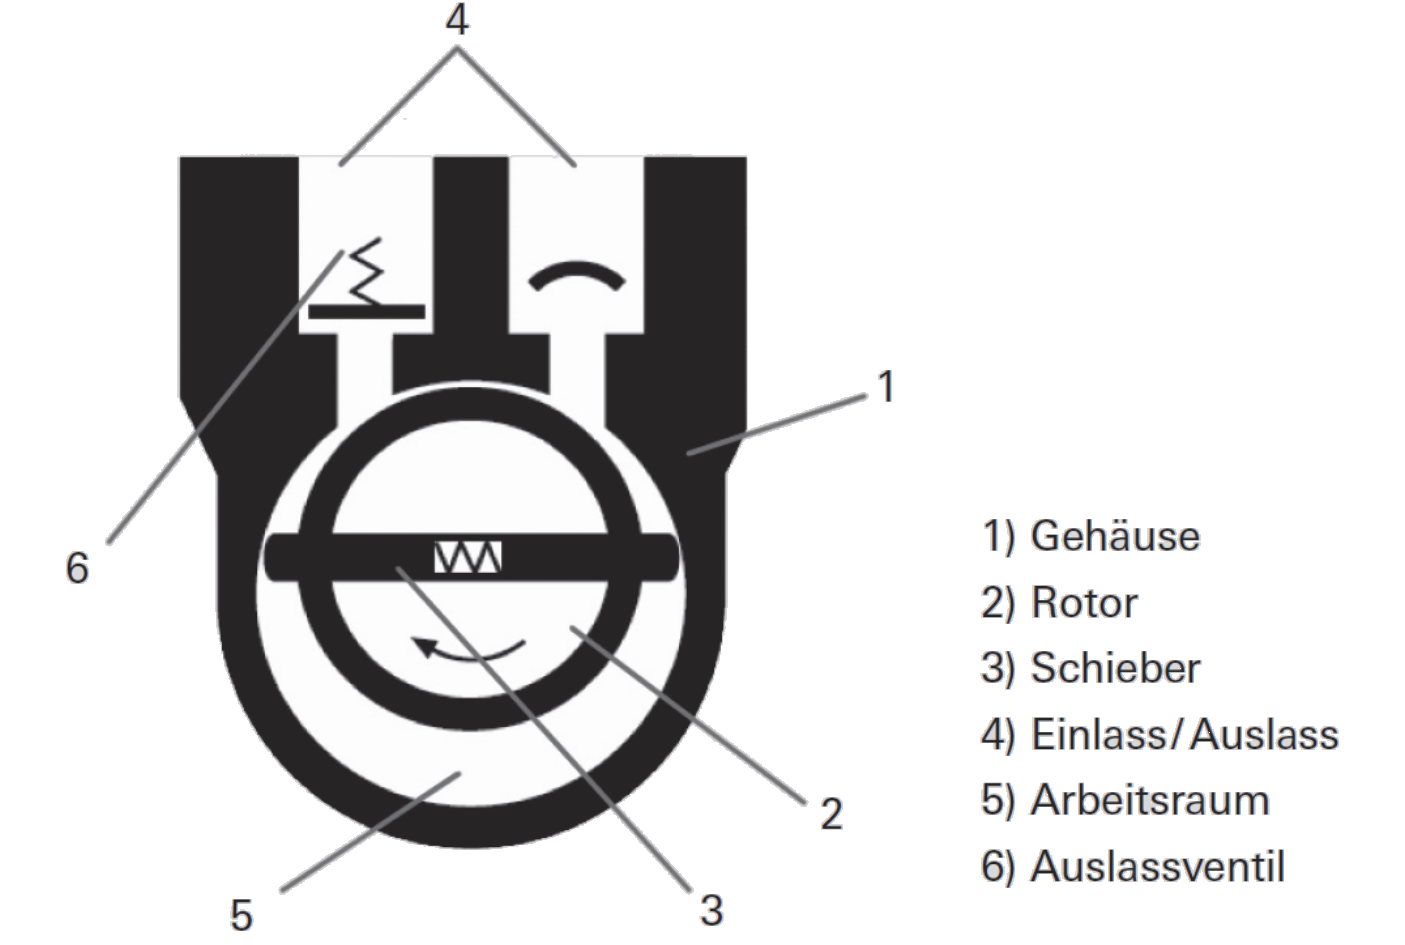
\includegraphics[scale=0.4]{Bilder/drehschieber.png}
  \caption{Schematische Darstellung des Aufbaus einer Drehschieberpumpe.\cite{schemadreh}}
  \label{drehschema}
\end{figure}

\subsubsection{Turbomolekularpumpe}
Die Turbomolekularpumpe besteht aus vielen beschaufelten Rotoren in einem zylinderförmigen Gehäuse. Die Gasmoleküle treffen auf die rotierenden Flächen und werden so kinetisch in Pumprichtung beschleunigt.
Aufgrund der hohen Rotationsfrequenz wird für den Betrieb einer Turbomolekularpumpe ein Vorvakuum benötigt, da anderenfalls die zufälligen Kollisionen der Gasmoleküle das Pumpen verhindern würden. Des Weiteren
könnte die Reibung der Gasmoleküle den Rotor beschädigen.
\\Zur Messung des erzeugten Vakuums werden im Verlauf des Versuchs drei unterschiedliche Messgeräte genutzt, welche hier beschrieben werden.
\subsubsection{Pirani-Messgerät}
Das Pirani-Messgerät wird für die höheren Druckbereiche ab $1000 \,\si{\milli\bar}$ genutzt. Die Funktionsweise dieser Messapparatur beruht auf der Tatsache, dass die Wärmeleitfähigkeit eines Gases von
dessen Druck abhängt. Zur Messung wird ein stromführender Glühdraht dem Vakuum ausgesetzt. Sinkt nun der Gasdruck, so steigt durch die verminderte Wärmeleitung des Gases die Temperatur des Drahtes.
Diese gesteigerte Temperatur verursacht eine Veränderung des Drahtwiderstandes, welcher über eine Brückenschaltung bestimmt werden kann. Es ist zu beachten, dass ein Pirani-Messgerät nur in einem
bestimmten Druckbereich anwendbar ist, da bei zu hohem Druck, die Konvektion die Wärmeleitfähigkeit des Gases überdeckt. Auf ähnliche Weise dominiert bei zu niedrigem Druck die Wärmestrahlung.
\subsubsection{Glüh- und Kaltkathoden Vakuummeter}
Das Glühkathoden Vakuummeter beruht auf der Ionisation der Gasmoleküle. Hierzu wird ein Glühdraht erhitzt, sodass durch thermische Elektronenemission Elektronen austreten, welche zu einer Anode
beschleunigt werden. Treffen die Elektronen auf ein Gasmolekül, so wird dieses durch das Herausschlagen eines Elektrons ionisiert. Das nun positiv geladene Gasteilchen lässt sich dann als
Ionisationsstrom messen. Zur Erhöhung der Trefferwahrscheinlichkeit der Elektronen, werden diese über ein Magnetfeld auf eine kreisförmige Bahn gebracht. Die Funktionsweise des Kaltkathoden-Vakuummeters
ist analog, jedoch werden hierbei die Elektronen durch ein starkes elektrisches Feld ausgelöst.
